\section{Player Enjoyment}
\label{chap:player_enjoyment}
The focus in this chapter is similar to the previous one, except that we will present data related to \textit{RQ3: How do game design elements and social interaction affect the players’ enjoyment in our game concept?} Chapter \ref{chap:discussion} will use this data to discuss and evaluate the results.

A player’s enjoyment in games is challenging to measure appropriately. Quantitative data from the application does not describe enjoyment in a good way. Thus, the primary data sources in this chapter are answers from the questionnaire and qualitative data from interviews and observations.

\subsection{Questionnaire}
Table \ref{tab:enjoyment_statements} summarizes the results from the nine statements related to the players’ enjoyment. As in the previous two chapters, the results use a three-point Likert scale for improved readability. The average answer from both research groups, student society (Avg S) and classmates (Avg C), are also presented.

\begin{table}[H]
    \centering
    \begin{tabularx}{\textwidth}{|c|X|c|c|c|c|c|}
        \hline
        & \multicolumn{1}{c|}{\textbf{Statements}}  & \multicolumn{1}{c|}{\textbf{Disagree}} & \multicolumn{1}{c|}{\textbf{Neutral}}  & \multicolumn{1}{c|}{\textbf{Agree}} & \multicolumn{1}{c|}{\textbf{Avg S}} & \multicolumn{1}{c|}{\textbf{Avg C}}\\ \hline
        \textbf{S17} & I liked the concept of Hover. & 10.53\% & 31.58\% & 57.89\% & 3.42 & 4.00 \\
        \textbf{S18} & It was sad to stop using Hover after the test period ended. & 36.84\% & 36.84\% & 26.32\% & 2.42 & 3.29 \\
        \textbf{S19} & I felt that the progress in the game was always clear. & 21.05\% & 26.32\% & 52.63\% & 3.17 & 3.86 \\
        \textbf{S20} & There was an appropriate degree of difficulty to achieve medals. & 21.05\% & 47.37\% & 31.58\% & 3.17 & 3.00 \\
        \textbf{S21} & My status in the game increased the more I played. & 10.53\% & 47.37\% & 42.11\% & 3.00 & 3.86 \\
        \textbf{S22} & The challenges I participated in had clear goals. & 0.00\% & 31.58\% & 68.42\% & 3.92 & 4.00 \\
        \textbf{S23} & I felt attached to my unique avatar. & 78.95\% & 5.26\% & 15.79\% & 1.33 & 2.71 \\
        \textbf{S24} & I was happy to get reactions to my activities and medals. & 26.32\% & 42.11\% & 31.58\% & 2.83 & 3.43 \\
        \textbf{S25} &  I was curious to see what my friends had been up to. & 52.63\% & 5.26\% & 42.11\% & 2.42 & 3.71 \\
        \hline
    \end{tabularx}
    \caption{Statements related to enjoyment.}
    \label{tab:enjoyment_statements}
    \vspace*{-\baselineskip}
\end{table}

Looking at the answers, we can see that the results are generally good, with a clear positive shift in many statements. A lot of the participants were either neutral or agreed. We find the first exception in S18, where the question was if it was sad to stop using Hover after the test period ended. The answers were more evenly distributed between the three possibilities; disagree, neutral, and agree. The most prominent deviation is S23, where most participants disagreed that they felt attached to their unique avatar. Additionally, there was a mix between users’ curiosity about what their friends had been doing in S25. Answers here had a clear overweight on the edge cases, either disagree or agree. S18 description?

The average numbers from the two different groups reveal a clear difference. There were generally more positive answers in the group of classmates than in the student society group. All statements except S20 had a higher average for the group consisting of classmates.

As part of the questionnaire, the respondents were asked if they had any additional comments related to their enjoyment. One of the respondents stated that it was satisfying to earn points, while another one enjoyed comparing points against friends:

\textit{“It was satisfying to earn points.”*}

\textit{“I enjoyed comparing my points against other people I knew.”*}

\begin{wrapfigure}{r}{0.45\textwidth}
    \vspace*{-\baselineskip}
    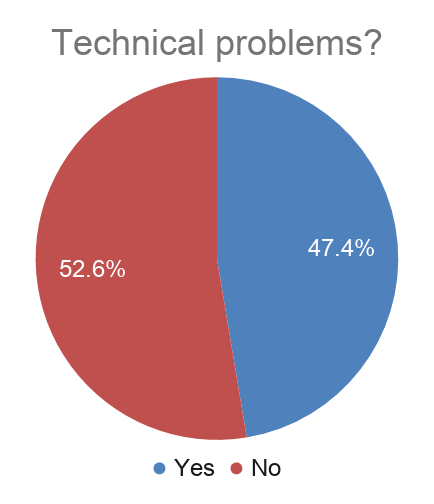
\includegraphics[width=0.7\textwidth, center]{Images/Results/TechnicalProblems.png}
    \caption{Share of people who had technical problems during the test period.}
    \label{fig:technical_problems}
    \vspace*{-\baselineskip}
\end{wrapfigure}

In addition to the statements directly related to enjoyment, answers from one of the general questions in the questionnaire are relevant to this topic. The participants were asked if they encountered any technical issues during the test phase. As seen in Figure \ref{fig:technical_problems}, almost half of the respondents answered “Yes.” Technical problems can result in frustration for players and thus decrease their enjoyment. An example is explained in a comment from one of the participants: 

\textit{“I lost the points I had earned one day because of a technical error, which made me sad.”*}

\subsection{Interviews}
In the interviews, we got some more insights into how the participants enjoyed the application. One of the participants thought it was a fun concept to try in an otherwise boring life, where many arrangements and meetings were canceled or postponed because of Covid-19.

Participants also mentioned that the social interaction between friends was something they enjoyed. Especially related to the “Hover with friends” functionality. Multiple interview subjects mentioned that they thought this part of the application was fun. According to one of the participants, whether or not people wanted to hover together was often a question.

However, not all enjoyment feedback brought up during the interviews was positive. Some participants reported aspects of the game that decreased their enjoyment. The most vital of these is related to the social part of the game. Multiple people mentioned that there should be a social system for categorizing friends and what the users see in the feed.

“I did not recognize all people publishing activities in the feed. Browsing the feed was, therefore, less fun.”*

Two of the interviewed participants also told us that they were forced to stay at home in the first week of testing. When they started to use the application, one week after everybody else, the enjoyment of hovering was less because they felt winning was unrealistic. One of them said:

“It was a bit depressing to see people earn points and get a head-start the week I was in quarantine.”*

\subsection{Observations}
Observations of players confirmed some of the aspects of players’ enjoyment revealed during the interviews. While observing people using the application, the social interaction seemed to cause the most enjoyment from the participants. People were talking about Hover and planning who should hover together. Apart from that, the observations did not reveal anything interesting related to the players’ enjoyment.

\subsection{Summary}
This chapter described results from the questionnaire, interview, and observations relevant to RQ4. The next chapter will continue presenting results from the survey and shift focus to the next research question (RQ5), investigating how Hover affected peoples’ habits.
